\section{Question 2}

\subsection{The Question}

\begin{flushleft}

Create an ASCII and JPEG dendrogram that clusters (i.e., HAC)
the most similar blogs (see slides 12 \& 13).  Include the JPEG in
your report and upload the ascii file to github (it will be too
unwieldy for inclusion in the report).

\end{flushleft}
\subsection{The Answer}

The Python function used to produce the ascii and jpeg dendrograms is provided in the book \cite{PCI}. The output of the script was redirected to a text file ``ascii.txt''. 

\lstset{
    language=Python,
    label=code:q1,
    caption={Python script to produce dendrograms}
}
\lstinputlisting{../q2/q2.py}

\begin{figure}
\centering
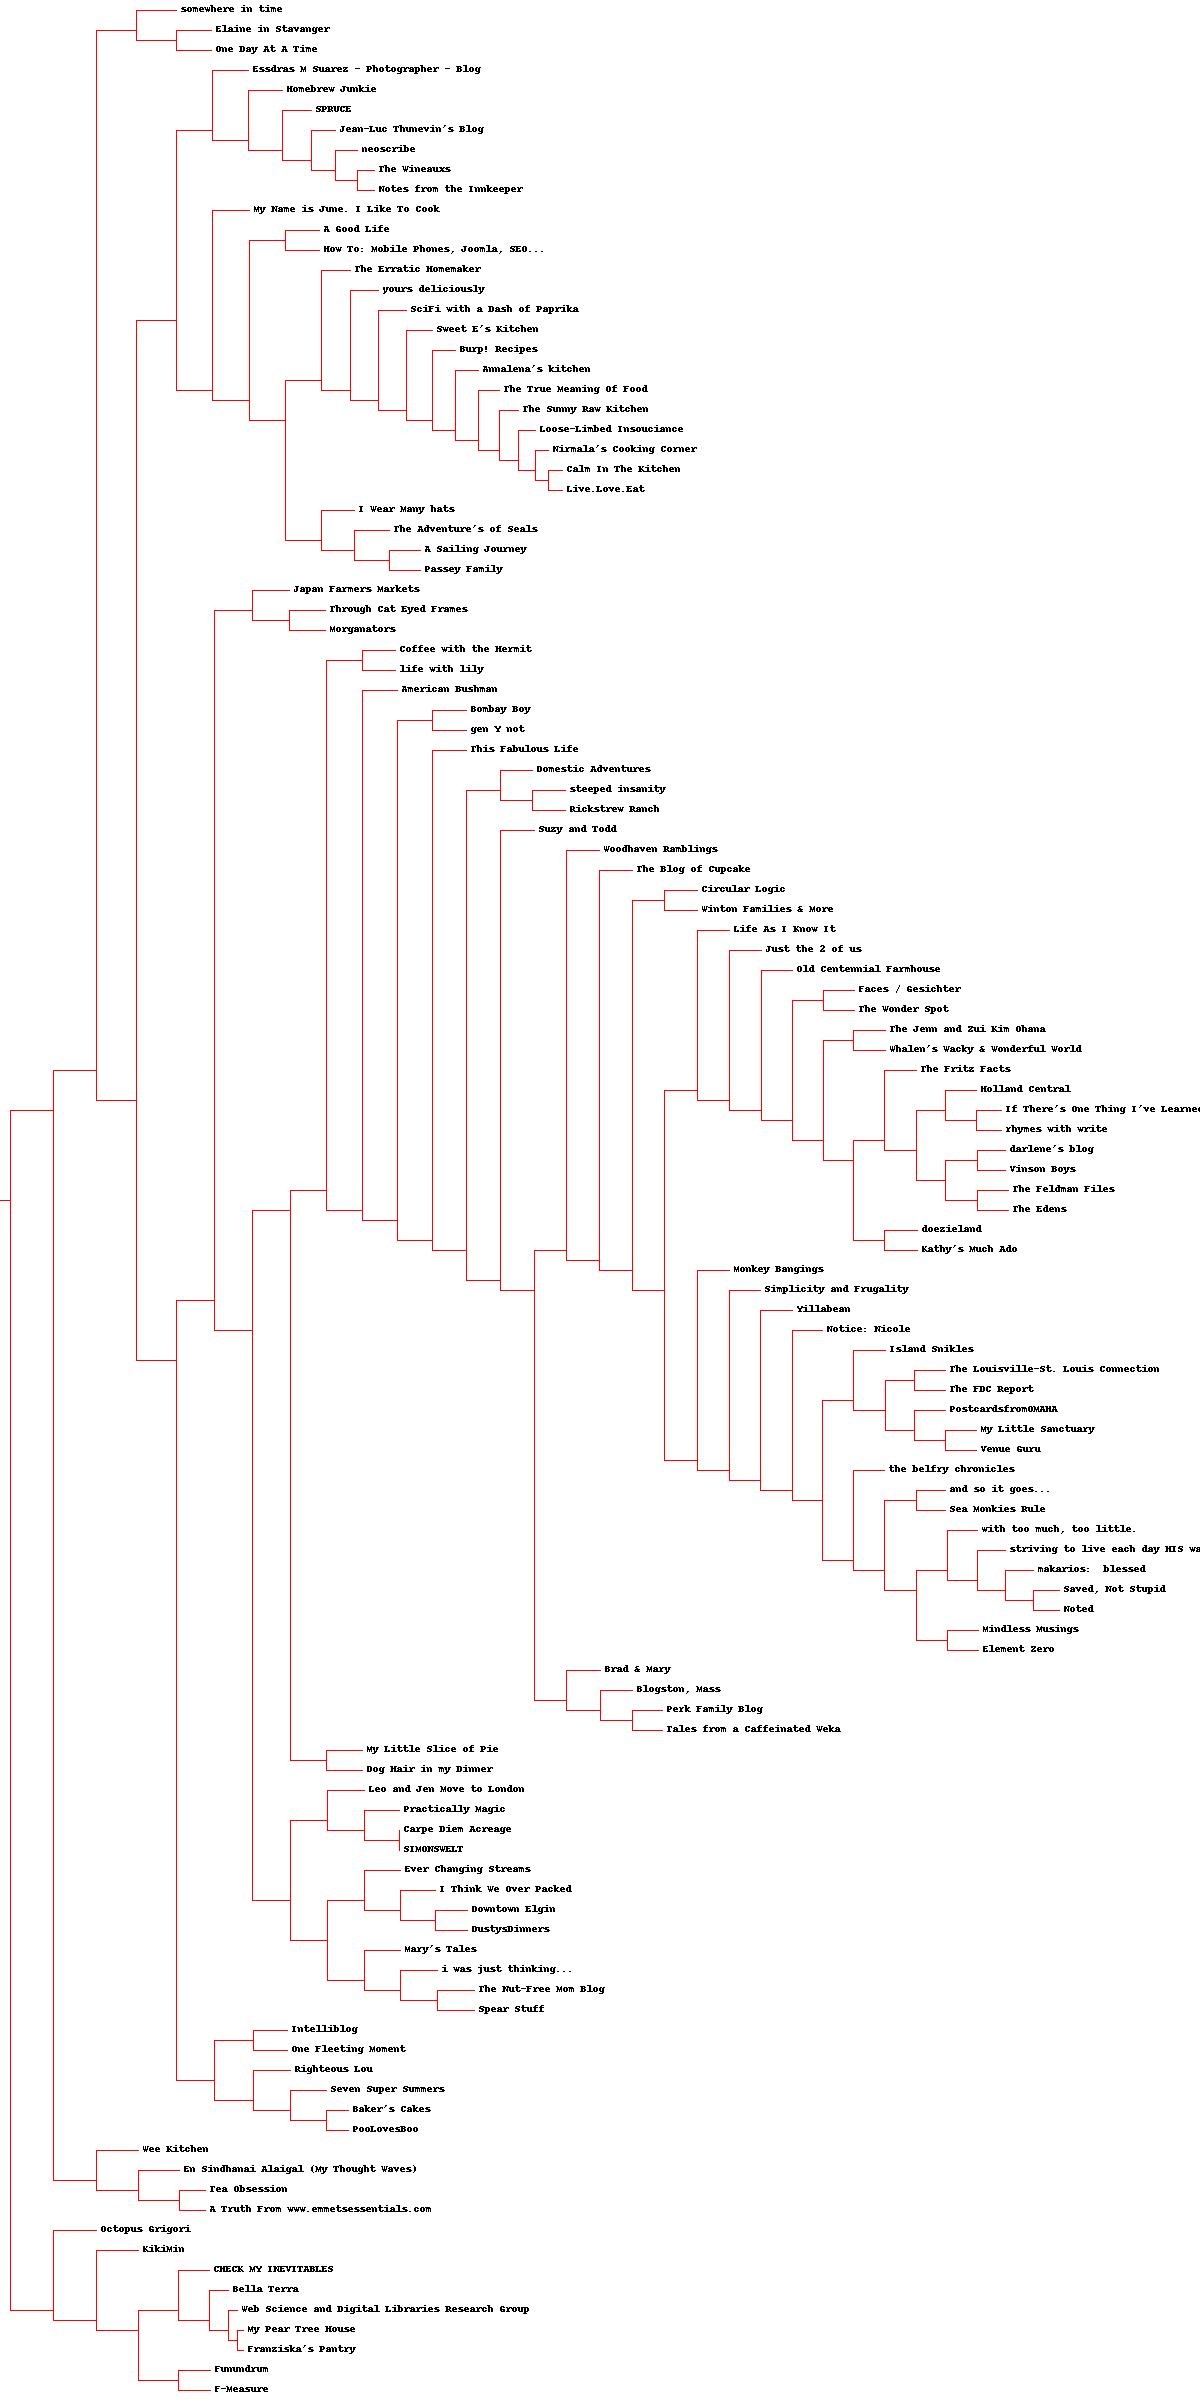
\includegraphics[height=25cm]{../q2/blogdendro.jpg}
\caption{JPEG dendrogram}
\end{figure}







